Um jogo pedag�gico utiliza-se de uma interface alg�brico-geom�trica do seguinte modo: os alunos devem eliminar os pontos do plano cartesiano dando "tiros", seguindo trajet�rias que devem passar pelos pontos escolhidos. Para dar os tiros, o aluno deve escrever em uma janela do programa a equa��o cartesiana de uma reta ou de uma circunfer�ncia que passa pelos pontos e pela origem do sistema de coordenadas. Se o tiro for dado por meio da equa��o da circunfer�ncia, cada ponto diferente da origem que for atingido vale 2 pontos. Se o tiro for dado por meio da equa��o de uma reta, cada ponto diferente da origem que for atingido vale 1 ponto. Em uma situa��o de jogo, ainda restam os seguintes pontos para serem eliminados: A(O; 4), 8(4; 4), C(4; O), 0(2 ; 2) e E(O ; 2).

\begin{figure}[h]
\centering
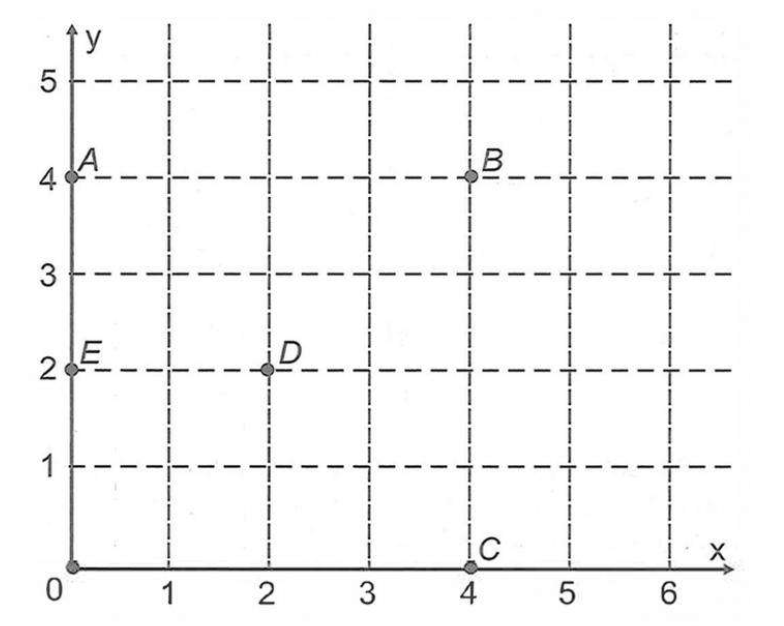
\includegraphics[width=8cm]{../figuras/q148-2018.png}
\end{figure}

\begin{enumerate}
\item[a)]x=0
\item[b)]y=0
\item[c)]$x^2+y^2=16$
\item[d)]$x^2+(y-2)^2=4$
\item[e)]$(x-2)^2+(y-2)^2=8$
\end{enumerate}